\documentclass[12pt]{report}
%================================================================
% Preamble declarations
%----------------------------------------------------------------

% This template was developed and maintained by John W. Shipman 
%   until his untimely passing in January 2017.
% If you have questions, please see the Center for Graduate Studies
%     2018/04/24 v11.0 Updated by L.M. Liebrock
%     2019/09/22 v12.0 Updated by A.I. El-Osery
%----------------------------------------------------------------
%
%
% Place \usepackage commands for other modules here
%%%%\usepackage{...}
\usepackage[sort&compress]{natbib}% Example bibliographic style
    % sort ... orders multiple citations into the sequence in which they appear in the list of references
    % sort&compress ... assort but in addition multiple numerical citations are compressed if possible (as 3–6, 15);

% Use the NMT 2020 thesis style
\usepackage{NMTthesis2023}
\usepackage[hypertexnames=false]{hyperref}  % create live links in TOC
    % options below control the color of links including urls, cite, etc. Feel free to change to your liking.
\hypersetup{
        colorlinks = true,
        linkcolor = black,
        anchorcolor = black,
        citecolor = black,
        filecolor = black,
        urlcolor = black,
	    pdfnewwindow = true,
        extension = pdf
} 
%----------------------------------------------------------------
%
% Select the type of publication, one of these three.
%
%----------------------------------------------------------------
%%%%\thesis
\dissertation
%%%%\mastersreport
%
%----------------------------------------------------------------
% General options
%
%----------------------------------------------------------------
% Enter "Your Name Here" as your full name  appears on your intent to graduate; this is how it will appear in all of the critical components of your document
\author{Your Name Here}

% Here your title is all in capital letters, but in ProQuest you are to enter it in Title Case. 
% need to use \protect\\ to do line breaks
\title{Place your title here, and use \protect\\
  commands to break lines}
  
\degreeSought{Doctor of Philosophy in Mechanical Engineering\\
  with Dissertation in Intelligent Energetic Systems}
 
% \degreeSought{Master of Science in Computer Science\\
%  with Specialization in Information Technology}
   
  
% Enter the date that you complete your thesis here.
\thesiscompletiondate{May 12, 2020}

% Enter the expected month and year for your degree conferral. This will be 
% two months after the thesis is completed and accepted in ProQuest, unless you complete for the May graduation deadline. 
\graduationdate{June, 2020}

%
% If you would like to give credit to a typist, uncomment this
% line and enter the typist's name
%
%%%%\typist{Rose Mary Woods and the author}

%----------------------------------------------------------------
%
% Name your academic advisor here.  Do not use titles such as Dr. or Ph.D.
%
\academicadvisor{Ada Lovelace}
%
% Use EITHER \researchadvisor or \coresearchadvisors ; comment out the other 
% Name your research advisor here.  Do not use titles such as Dr. or Ph.D.
%
\researchadvisor{Ada Lovelace}
%\coresearchadvisors{Ada Lovelace}{Grace Hopper}
%
%
% Number of people on your committee including academic and research advisor(s); Replace "6" with the number for your committee
%
\committeesize{3}

% Name your committee members (not including research advisor(s)) for your approvals page

% Note committee members will be printed in the order listed, not numerical order
%  Do not use titles such as Dr. or Ph.D.
%
\committeememberone{Committee Member 1}
\committeemembertwo{Committee Member 2}
\committeememberthree{Committee Member 3}
\committeememberfour{Committee Member 4}
\committeememberfive{Committee Member 5}
%
%
%================================================================
\begin{document}
%
% Begin front matter
%
%----------------------------------------------------------------
%
% Produce the title page
%
\titlepage
%----------------------------------------------------------------
%----------------------------------------------------------------
%%%%\epigraph[who said it]{what they said}


%----------------------------------------------------------------
%%%%\frontispiece[title of the graphic]{some graphic}
%----------------------------------------------------------------


%----------------------------------------------------------------
\begin{dedication}
This thesis is dedicated to...
\end{dedication}



%----------------------------------------------------------------
\begin{acknowledgments}

\end{acknowledgments}
%----------------------------------------------------------------
%
% An abstract is required.  
% After your abstract, provide two to six keywords, or key 
% phrases of up to three words, to assist librarians in
% indexing your work.
%
\begin{abstract}

From experts with the International Studies Association, recommendations suggest
making this your "elevator pitch" to concisely summarize your work including its
broader implications to "convey the academic triangle of theorizing, method, and
data".  Here are a few tips from the American Journal Experts: 1. write your
thesis first, 2. briefly use background information to lead to your aim, 3.
outline your methodology, 4. describe your most important findings, 5. state
your conclusions, but avoid overstatement. Remember to be concise and have other
people  review the abstract for clarity

\keywords{Keyword1; Keyword2; Key Phrase 3; ...}
\end{abstract}

%----------------------------------------------------------------
%\signaturepage
\tableofcontents
%
% If you have no tables, comment out \listoftables.
%
\listoftables
%
% if you do not have figures, comment out the following lines
\listoffigures
%{
%\let\oldnumberline\numberline%
%\renewcommand{\numberline}{\figurename~\oldnumberline}
%\listoffigures
%}

%%%%\listofabbrs
% If you provide a List of Abbreviations, create a file
%   'abbrs.tex' containing the abbreviations table and
%    uncomment the following line
% 
%\listofabbrs
%
%----------------------------------------------------------------
\signaturepage
%----------------------------------------------------------------
%%%%\begin{preface}
%%%%
%%%%\end{preface}
%================================================================
% Body of the document.   Use one of these commands to start each
% chapter:
%   \chapter{FIRST CHAPTER TITLE}
%   \chapter[FIRST SHORT TITLE]{FULL LENGTH CHAPTER TITLE}
% If you have appendices, use these commands:
%   \appendix
%   \chapter{FIRST APPENDIX TITLE}
%     ...
%   \chapter{SECOND APPENDIX TITLE}
%     ...
%----------------------------------------------------------------
\chapter{Test READ BEFORE REPLACING THIS\protect\\ CHAPTER WITH YOUR CONTENT}
When you are getting ready to write your thesis, you may want to consider taking the Thesis and Dissertation Bootcamp that is offered as a one credit class before the spring semester each year. Contact the CLASS department if you have questions on the course, which provides instruction, then has you focus on writing one or more chapters of the thesis/dissertation. You must apply for taking this class in the fall with a plan that is developed by you and your advisor.

As you write your thesis, make sure that you properly quote, paraphrase, and cite your sources. If you need assistance, the Writing and Oral Presentation Center and the STEM Communication Fellows can help you with this aspect and reviewing your work. Here is an example of citing a reference~\cite{Brown1997}. Or you can list multiple~\cite{ElSheimy2008,El-Diasty2009}.

If you use a significant resource from another source, e.g., a conference or journal paper, you must have permission from the copyright holder, i.e., the journal, to reuse the resource. Examples of such significant resources are figures, tables, and long quotations. The last appendix is the where you put these permissions, where are to list what in your document you have gotten permission for and the permission you received. It is recommended that you get these permissions when you add a resource rather than waiting until the last minute. 
\chapter{SECOND CHAPTER TITLE}
\section{Section Title}
\subsection{Subsection Title}
Paragraph 1

Table \ref{table:1} is an example of referenced \LaTeX elements.
 
\begin{table}[h!]
\centering
\begin{tabular}{||c c c c||} 
 \hline
 Col1 & Col2 & Col2 & Col3 \\ [0.5ex] 
 \hline\hline
 1 & 6 & 87837 & 787 \\ 
 2 & 7 & 78 & 5415 \\
 3 & 545 & 778 & 7507 \\
 4 & 545 & 18744 & 7560 \\
 5 & 88 & 788 & 6344 \\ [1ex] 
 \hline
\end{tabular}
\caption{Table to test captions and labels}
\label{table:1}
\end{table}


Paragraph 2
\begin{figure}[ht]
\centering

\includegraphics[width=3.5in]{nmt.jpg}
\caption[captiontext]{this is the text of your caption.}\label{figure:1}
\end{figure}

Paragraph 3
\begin{figure}[ht]
\centering
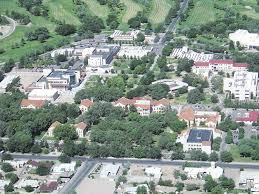
\includegraphics[width=3.5in]{nmt_campus}
\caption[captiontext]{this is the text of your caption.}\label{figure:2}
\end{figure}

%================================================================
% References section.  
%\bibliographystyle{apalike}
\bibliographystyle{unsrt}
\bibliography{references}

%================================================================
% Appendices section.  
% If you don’t have appendices, comment out these lines
   \appendix
   \chapter{1st app TITLE}
   \section{First section of Appendix A}
%     ...
   \chapter{SECOND app TITLE}
%     ...
%  READ PERMISSIONS BEFORE COMMENTING OUT OR REMOVING
\chapter{PERMISSIONS}
   This is your last appendix. 
   
   Place all of your permissions here for everything used from copyrighted material: i.e., long quotations, tables, and figures. Label each permission page with the list of figure numbers or tables or sections of your text that is from the copyrighted material.
   
   Most journals have an online permissions process where you submit what you are using from the journal and an automatic system sends you permissions for a thesis/dissertation OR they have a blanket permission for use in a thesis/dissertation. 
   
   You must have permission for your own published work when you have signed a copyright release form; the above description for journals applies here as well. 
   
   If you are using material from an NMT thesis or dissertation, you may use the permission page at the end of the referenced thesis as your permission. 
%     ...


% 
\copyrightpage

\end{document}
